Platforma społecznościowa Meetup, założona w 2002 roku, stanowi istotne narzędzie umożliwiające ludziom integrację wokół wspólnych zainteresowań. Oferuje użytkownikom narzędzia do tworzenia grup, organizowania wydarzeń oraz nawiązywania kontaktów z innymi osobami o podobnych pasjach. Jest to bezpłatna platforma, dostarczająca rozległego zestawu funkcji, które pozwalają na sprawną organizację i zarządzanie różnorodnymi wydarzeniami. \autocite{meetup}

Użytkownicy mają zdolność tworzenia zarówno wydarzeń online, jak i offline, precyzyjnie określając datę, godzinę oraz lokalizację spotkania. Dodatkowo, mają możliwość wysyłania zaproszeń do potencjalnych uczestników. Meetup oferuje zróżnicowane narzędzia do skutecznego zarządzania wydarzeniami, co obejmuje m.in. funkcję rejestracji uczestników, zbieranie płatności oraz wysyłanie powiadomień.

W przedstawionym na \autoref{rys:meetup_interfejs} interfejsie użytkownika platformy Meetup dla uczestnika wydarzenia uwidacznia się kompletność informacyjna, obejmująca nazwę wydarzenia, datę, godzinę, lokalizację oraz opis wydarzenia.
\begin{figure}[H]
    \begin{center}
    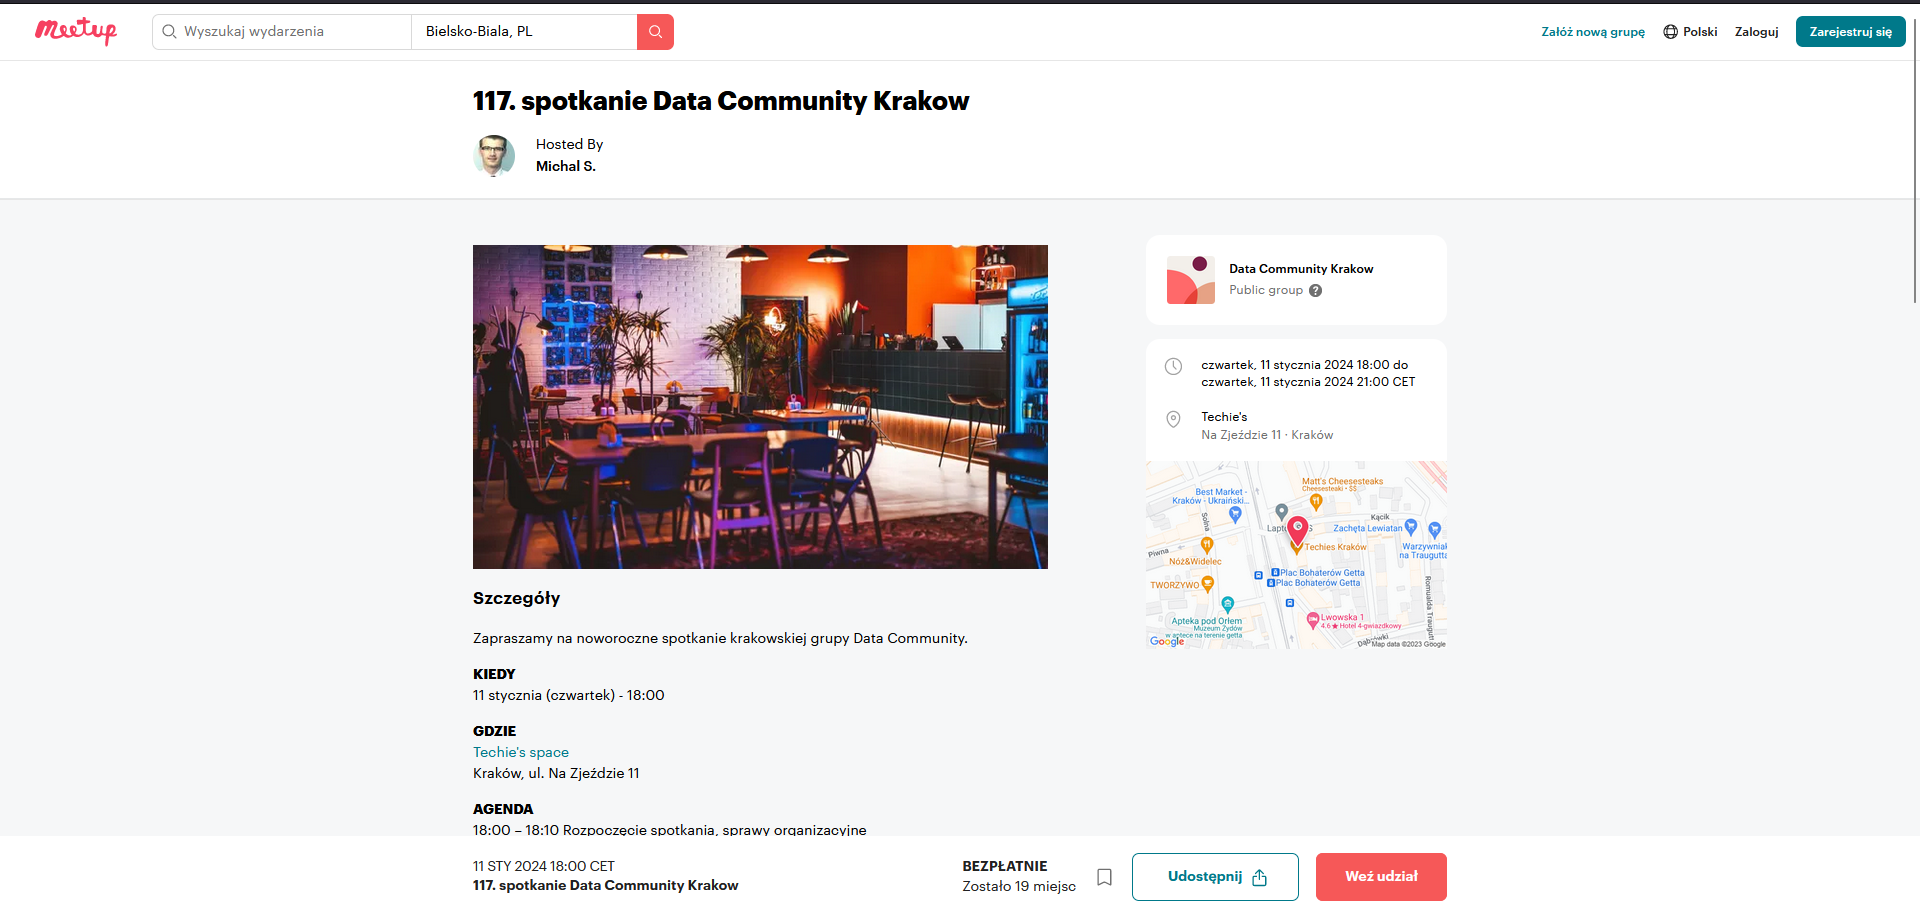
\includegraphics[scale=0.35]{imgs/solutions/meetup.png}
    \end{center}
    \caption{Strona informacyjna o wydarzeniu w serwisie Meetup}
    \label{rys:meetup_interfejs}
    \end{figure}